\documentclass[tikz,border=10pt]{standalone}
\usepackage[utf8]{inputenc}
\usepackage[T1]{fontenc}
\usepackage{amsmath,amssymb}
\usepackage{tikz}
\usetikzlibrary{shapes.geometric, arrows.meta, positioning, calc, fit, backgrounds}

\definecolor{primary}{HTML}{0F172A}
\definecolor{primaryblue}{HTML}{1E3A8A}
\definecolor{accentblue}{HTML}{0284C7}
\definecolor{tealaccent}{HTML}{0D9488}
\definecolor{darkgreen}{HTML}{065F46}
\definecolor{lightgreen}{HTML}{ECFDF5}
\definecolor{crimson}{HTML}{991B1B}
\definecolor{lightred}{HTML}{FEF2F2}
\definecolor{amber}{HTML}{B45309}
\definecolor{lightamber}{HTML}{FFFBEB}
\definecolor{boxbg}{HTML}{F8FAFC}

\begin{document}

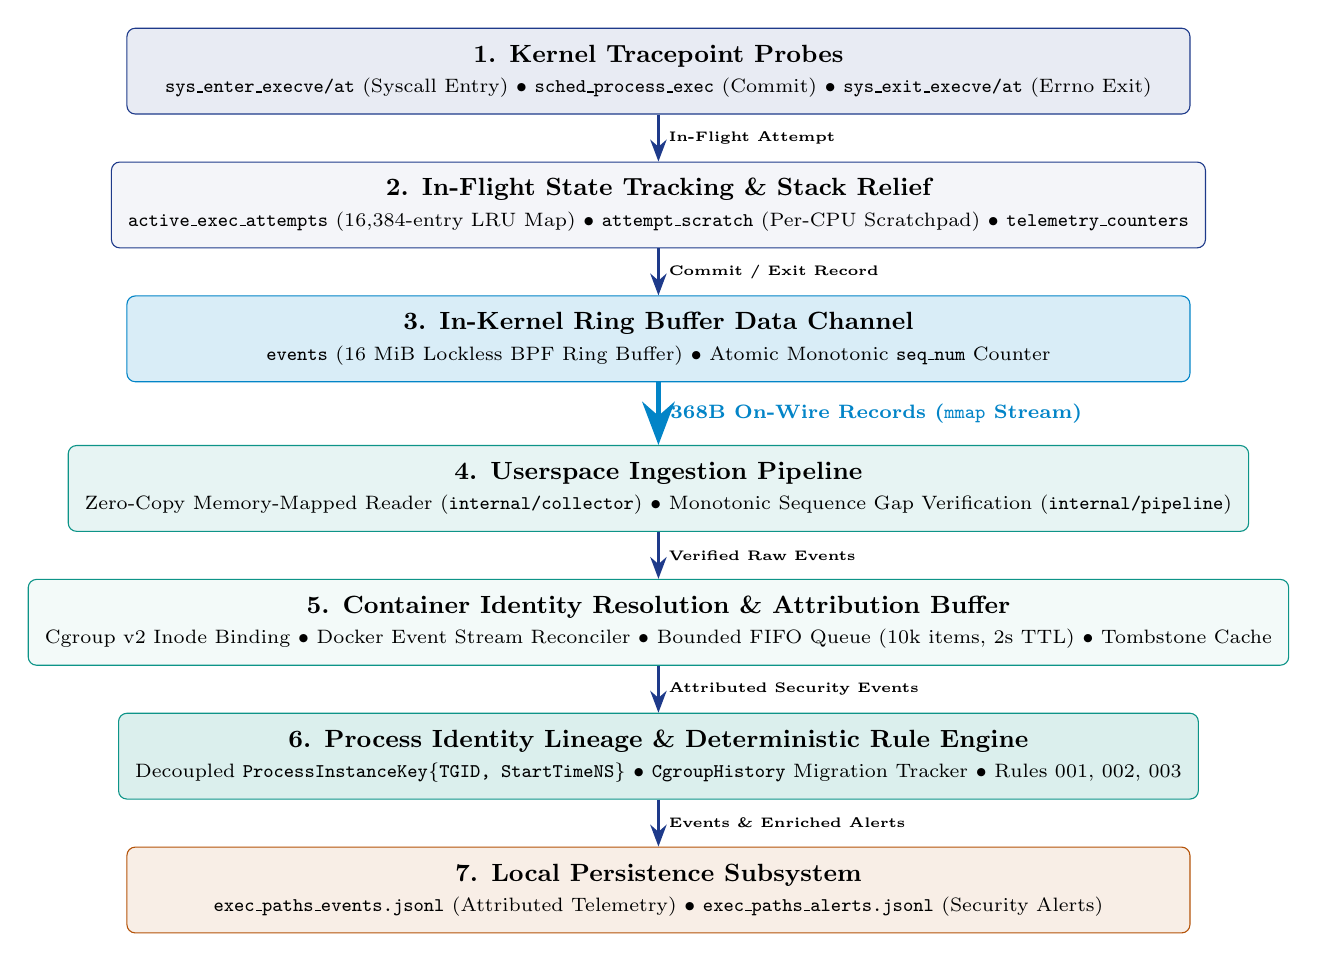
\begin{tikzpicture}[
    tierbox/.style={rectangle, draw=primaryblue, fill=primaryblue!10, rounded corners=3pt, font=\small\bfseries, align=center, inner sep=6pt, minimum width=13.5cm, minimum height=0.9cm},
    userbox/.style={rectangle, draw=tealaccent, fill=tealaccent!10, rounded corners=3pt, font=\small\bfseries, align=center, inner sep=6pt, minimum width=13.5cm, minimum height=0.9cm},
    storebox/.style={rectangle, draw=amber, fill=amber!10, rounded corners=3pt, font=\small\bfseries, align=center, inner sep=6pt, minimum width=13.5cm, minimum height=0.9cm},
    arrow/.style={-{Stealth[scale=1.2]}, thick, draw=primaryblue},
    thickflow/.style={-{Stealth[scale=1.3]}, line width=2pt, draw=accentblue}
]
    \node[tierbox] (t1) at (0, 7.5) {1. Kernel Tracepoint Probes\\ \scriptsize\textnormal{\texttt{sys\_enter\_execve/at} (Syscall Entry) $\bullet$ \texttt{sched\_process\_exec} (Commit) $\bullet$ \texttt{sys\_exit\_execve/at} (Errno Exit)}};
    \node[tierbox, fill=primaryblue!5] (t2) at (0, 5.8) {2. In-Flight State Tracking \& Stack Relief\\ \scriptsize\textnormal{\texttt{active\_exec\_attempts} (16,384-entry LRU Map) $\bullet$ \texttt{attempt\_scratch} (Per-CPU Scratchpad) $\bullet$ \texttt{telemetry\_counters}}};
    \node[tierbox, draw=accentblue, fill=accentblue!15] (t3) at (0, 4.1) {3. In-Kernel Ring Buffer Data Channel\\ \scriptsize\textnormal{\texttt{events} (16 MiB Lockless BPF Ring Buffer) $\bullet$ Atomic Monotonic \texttt{seq\_num} Counter}};

    \node[userbox] (t4) at (0, 2.2) {4. Userspace Ingestion Pipeline\\ \scriptsize\textnormal{Zero-Copy Memory-Mapped Reader (\texttt{internal/collector}) $\bullet$ Monotonic Sequence Gap Verification (\texttt{internal/pipeline})}};
    \node[userbox, fill=tealaccent!5] (t5) at (0, 0.5) {5. Container Identity Resolution \& Attribution Buffer\\ \scriptsize\textnormal{Cgroup v2 Inode Binding $\bullet$ Docker Event Stream Reconciler $\bullet$ Bounded FIFO Queue (10k items, 2s TTL) $\bullet$ Tombstone Cache}};
    \node[userbox, fill=tealaccent!15] (t6) at (0, -1.2) {6. Process Identity Lineage \& Deterministic Rule Engine\\ \scriptsize\textnormal{Decoupled \texttt{ProcessInstanceKey\{TGID, StartTimeNS\}} $\bullet$ \texttt{CgroupHistory} Migration Tracker $\bullet$ Rules 001, 002, 003}};

    \node[storebox] (t7) at (0, -2.9) {7. Local Persistence Subsystem\\ \scriptsize\textnormal{\texttt{exec\_paths\_events.jsonl} (Attributed Telemetry) $\bullet$ \texttt{exec\_paths\_alerts.jsonl} (Security Alerts)}};

    \draw[arrow] (t1) -- node[right, font=\tiny\bfseries]{In-Flight Attempt} (t2);
    \draw[arrow] (t2) -- node[right, font=\tiny\bfseries]{Commit / Exit Record} (t3);
    \draw[thickflow] (t3) -- node[right, font=\scriptsize\bfseries\color{accentblue}]{368B On-Wire Records (\texttt{mmap} Stream)} (t4);
    \draw[arrow] (t4) -- node[right, font=\tiny\bfseries]{Verified Raw Events} (t5);
    \draw[arrow] (t5) -- node[right, font=\tiny\bfseries]{Attributed Security Events} (t6);
    \draw[arrow] (t6) -- node[right, font=\tiny\bfseries]{Events \& Enriched Alerts} (t7);
\end{tikzpicture}

\end{document}
